\documentclass[10pt,a4paper]{article}
\usepackage[margin=2.2cm]{geometry}
\usepackage{fontspec}
\usepackage{kotex}
\setmainfont{Apple SD Gothic Neo}
\setsansfont{Apple SD Gothic Neo}
\usepackage{amsmath,amssymb}
\usepackage{graphicx}
\usepackage{booktabs}
\usepackage{caption}
\usepackage[dvipsnames]{xcolor}
\usepackage[colorlinks=true,linkcolor=MidnightBlue,citecolor=MidnightBlue,
            urlcolor=MidnightBlue]{hyperref}
\usepackage{titlesec}
\titleformat{\section}{\large\bfseries}{\thesection}{0.6em}{}
\titleformat{\subsection}{\normalsize\bfseries}{\thesubsection}{0.5em}{}
\captionsetup{font=small,labelfont=bf}
\setlength{\parskip}{0.35em}
\setlength{\parindent}{0pt}

\usepackage{mdframed}
\newmdenv[linewidth=0.4pt,linecolor=gray!60,backgroundcolor=gray!5,
          innertopmargin=6pt,innerbottommargin=6pt,skipabove=8pt,skipbelow=8pt]{claimbox}
\newcommand{\claim}[2]{\begin{claimbox}\textbf{주장.} #1\par\smallskip
  \textcolor{gray!70}{\textbf{반증 조건.} #2}\end{claimbox}}

\title{\bfseries 오십 건\\[2pt]
\large 봉인 도메인의 적응 곡선 --- 전이는 자료가 없을 때의 다리다}
\author{월드모델 실험실 · 노트 $815$}
\date{2026-08-07}
\begin{document}\maketitle

\section{한 줄}

사용자 로드맵의 재정의 --- \emph{``zero-shot 을 적응 곡선으로 보라. $n{=}0$
절편·기울기·포화점이 곧 온보딩 가격표''} --- 를 \textbf{진짜 봉인 도메인}에서
실측했다. KR 만화 $1{,}716$행은 판이 한 줄도 학습하지 않았고, $n{=}0$ 절편(챔피언
전이)은 이미 재 있었다.

\begin{center}
\begin{tabular}{lrr}
\toprule
& 평가 $500$행 스피어만 & \\
\midrule
$n{=}0$ (챔피언 전이) & $0.6877 \pm 0.0109$ & 절편 \\
$n{=}5$ & $0.336$ & 축 $4$개의 정보만으로 \\
$\mathbf{n^{*}{=}50}$ & $0.684$ & \textbf{전이와 동급} \\
$n{\geq}100$ (고원) & $\mathbf{0.752}$ & \textbf{전이 $+0.065$ 위} \\
\bottomrule
\end{tabular}
\end{center}

판정(번호 우선순위 · 두 번째 이행 · 충돌 없음): \textbf{3.교차, $n^{*}=50$.}

\begin{figure}[t]\centering
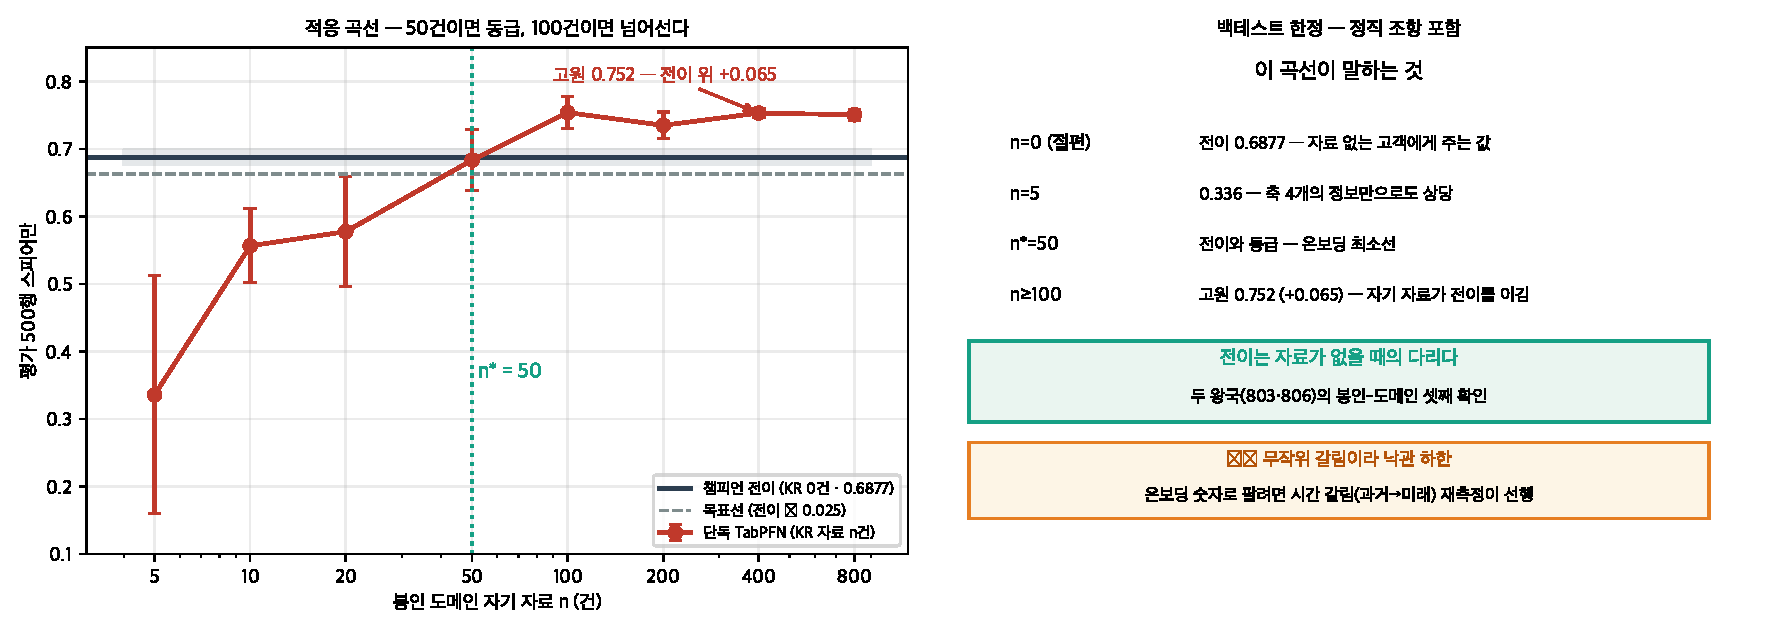
\includegraphics[width=0.97\textwidth]{figs/adapt.pdf}
\caption{왼쪽: 곡선과 세 선(전이·목표·$n^{*}$). 오른쪽: 읽는 법과 정직 조항.}
\end{figure}

\section{고원이 전이 위에 있다}

\claim{\textbf{전이는 자료가 없을 때의 다리다.} $n \geq 100$ 부터 자기 자료
단독(TabPFN)이 $11$도메인 합동 전이를 $+0.065$ 넘어선다 --- 논문 $167 \cdot
170$ 의 ``두 왕국''이 봉인 도메인에서 세 번째로 확인됐다: 전이가 이기는 곳은
자기 정보가 없는 곳이고, 정보가 서면($100$건) 자기 자료가 이긴다. \textbf{온보딩
문장(백테스트 한정)}: 과거 $50$건이면 우리 전이와 동급 · $100$건이면 그 위 ---
사용자가 말한 ``락인''의 실측 근거이기도 하다(고객 자료가 쌓일수록 그 고객
전용 정확도가 전이를 넘는다).}
{\textbf{무작위 갈림이라 낙관 하한이다.} 적응 팔은 같은 시대 분포의 $n$ 건을
본다 --- 실제 온보딩은 과거$\to$미래라 시간 이동 비용이 빠져 있다. 전이
기준선도 같은 평가 $500$ 이라 \textbf{상대 비교는 공정}하지만, $n^{*}$ 를
숫자로 팔려면 \textbf{시간 갈림 재측정이 선행}이다(T$1$ 다음 실험으로 등록).}

\section{예측 채점}

교차 적중(주 갈래) · $n^{*}$ 는 내 구간 $[100,400]$ 밖($50$ --- 좋은 쪽) ·
$n{=}5$ 절편 $0.336 \in [0.1, 0.35]$ 적중. 갈래 번호 우선순위가 두 번째로 충돌
없이 작동했다. 판 $\rho$ $0.4689$ 그대로.

\end{document}
